\textit{In this chapter, we cover the RQ4 having a practical case with DBpedia improving the quality of the identifiers in order to better relate the datasets. We approach a problem where the DBpedia dataset has multiple URIs within the dataset and from other datasets connected with (transitive) \qname{owl:sameAs} relations and thus referring to the same concepts.
With this heterogeneity of identifiers it is complicated for users and agents to find the unique identifier which should be preferably used.
We are introducing the concept of DBpedia Unique Identifier (DUI) and a dataset of linksets relating URIs to DUIs.
In order to improve the quality of our dataset we developed a mechanism that allows the user to rate and suggest links.
% The DBpedia sameAs service further provides a web user interface for retrieving and rating the DUIs.
As proof of concept an implementation with a graphical web user interface is provided for accessing the linkset and rating the links.
The DBpedia sameAs service is available at \url{http://dbpsa.aksw.org/SameAsService}.}

\subsection{The DBpediaSameAs approach}

%Firstly, the meaning of things is an appropriated start, 

%Why does this problem occurs?
%First paragraph: motivation
As DBpedia~\cite{dbpedia-swj} was evolving during the 9 years of its existence, the community extended the linksets to DBpedia resources.
Thus, DBpedia has more than one URI that represents the same resource, which leads to the identifier heterogeneity problem. 
For instance a DBpedia resource can contain \qname{owl:sameAs} links to other data sets such as FreeBase\footnote{Freebase project webpage: \url{http://freebase.com}}, Wikidata, GeoNames\footnote{GeoNames project and exploration webpage: \url{http://geonames.org}} or yago\footnote{Yago project webpage:\url{http://yago-knowledge.org}}.
%Therefore the resource identification can not be achieved using \qname{owl:sameAs} links exclusively.
%but this mechanism is able to be improved in specifics cases, e.g. with the DBpedia \footnote{\url{http:dbpedia.org}}.

Further DBpedia has more than one URI representing the same resource within the dataset, e.g. the \qname{dbpedia:Brassil} has at least the following equivalents within the DBpedia \qname{dbpedia:Republica_Federativa_do_Brasil}, \qname{dbpedia:ISO_3166-1:BR} and \qname{dbpedia:Brazil} which are all redirecting to \qname{dbpedia:Brazil}.
Thus a problem to consider is to directly resolve any of the equivalents directly to the final URI e.g. \url{http://dbpedia.org/resource/Brazil} without any redundancies.

% from \textit{freebase.com} like \url{http://rdf.freebase.com/ns/m.015fr}

Also, according to Halpin et. al. \cite{DBLP:conf/semweb/HalpinHMMT10} and Wood et. al. \cite{dwood2014}, \textit{sameas.org} has collected millions of triples with \qname{owl:sameAs} relations.
It would be important to promote reciprocal owl:sameAs confirmation mechanisms and develop effective trust mechanisms to assure the quality of \qname{owl:sameAs} relations.


%According Wood et al. \cite{dwood2014}, several \qname{owl:sameAs} triples have been collected using sameAs.org \footnote{\url{http://sameAs.org}},  and the book recommends that you should get into the habit of checking that site before you make your own vocabulary or publish new \qname{owl:sameAs} triples.

%Thus, the results from the website sameAs.org, that e.g. brings more than 1140 results of \qname{owl:sameAs} occurrences for one URI, but the purpose of the sameAs.org stay on the right way, because he was created to bring occurrences of \qname{owl:sameAs} around the Internet, and our work is not a comparison with sameAs.org, but just a short example, our work focuses only in DBpedia resources rather than sameAs.org. 


%description of approach
% To tackle the identifier heterogeneity problem we introduce an approach for the link normalization, which also incorporates user feedback about the quality of links.
% Our approach utilizes DBpedia Unique Identifiers (DUI) for the DBpedia resources and can be applied for avoiding \qname{owl:sameAs} transient and redundant links in a DBpedia Link Repository. 

%mitigation = reduction (http://www.thesaurus.com/browse/mitigation?s=t)
To tackle the identifier heterogeneity problem we are making the following contributions:
\begin{itemize}
\item We describe an approach for the mitigation of the identifier heterogeneity problem and implement a prototype where the user is able to evaluate existing links, as well as suggest new links to be rated.
\item The ability to generate statistics about good and bad links which, brings the possibility to have a quality control for the links to DBpedia. %, which helps to improve the repository. 
\item We define the DBpedia Unique Identifier (DUI), which instead of several transient \qname{owl:sameAs} DBpedia URIs for the same final address, now is possible to have a unique URI from DBpedia.
A DUI goes directly to the final address instead of having to process several possible intermediate results.
For example, with a URI from \textit{Freebase}, 17 redundant URIs from DBpedia where avoided or if one used a service such as sameAs.org, 1141 URIs would be avoided.

\end{itemize}

The rest of the chapter is organized as follows: 
section \ref{representationidea} represents a proposed approach for tackling the identifier heterogeneity problem and section \ref{ev:dbpediasameas} we evaluate our work.


\subsection{Representation of the idea}\label{representationidea}

This section provides an explanation about our main idea, such as implementation and descriptions.

Before continuing the work, there are some definitions that were adopted.
\begin{itemize}
\item  \textbf{Normalization of the URI}: Is understood by normalizing URIs, the fact of eliminating redundancies.

\item \textbf{DBpedia unique identifier}: The DBpedia Unique Identifier (DUI) is an unique URI that identifies a resource in the DBpedia repository and also is the result of our normalization.
\end{itemize}

The idea started with a stand alone service on the web that solves the problem where the user provides a URI as parameter and instead of several transient URIs with \qname{owl:sameAs} property, the user receives a single DUI from our service.

\subsection{The work-flow}
The work-flow for requesting the DUI of a given resource is represented in  figure \ref{fig:generalworkflow}.
Firstly, the user will provide a URI from some address, i.e. FreeBase. Then, instead of possible several results of URIs with the property \qname{owl:sameAs}, our system will return a DUI. Consequently, the user has a possibility to rate, verify, validate, and suggest a different link. Then the rate can give us a chance to have statistics about the quality of the links.

\begin{figure}[hbt] 
  	\centering
	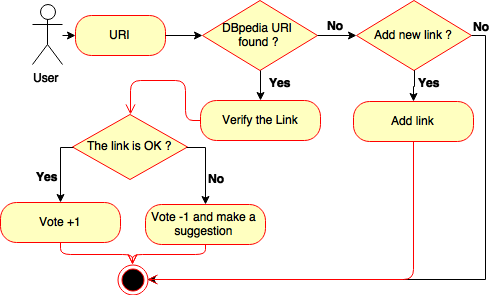
\includegraphics[width=\columnwidth]{img/generalFlow.png}
 	\caption{General work-flow.}
  	\label{fig:generalworkflow}
\end{figure}

A service, also was implemented, where the user can provide a URI and the API will return the DBpedia identifier like a URI that represents the \qname{owl:sameAs} about the URI provided.

\subsection{Methodology}
This section describes in four steps the technique and how the idea was developed, from phase of importing links to a relational database until the development of the service on the web and a GUI.

(1) The files with triples that contains \qname{owl:sameAs} links, were downloaded.
(2) All triples were imported in a relational database \footnote{Link to the database: \url{http://tinyurl.com/creatdb}}, because we will use some characteristics of a relational database i.e. comparative with voting system in future works.
(3) An implementation of a service on the web was provided, where the user enters the URI and receives a DUI.
(4) In order to provide an interface to access this service were created a web system that receive as input a URI, return as output an DBpedia identifier and allow rate and make suggestions about the resulting link.

%This paper provides an approach that will work on the problem of how to tackle heterogeneity searching for \qname{owl:sameAs} occurrences that were observed during a finding of co-references between different data sets. As a contribution to face this problem, a normalization about URIs was implemented in the context of the DBpedia resources. Thus, was developed a proof of concept in a computer software that implement an alternative contextual solution. 

figure \ref{fig:contrib} presents the relation of the contribution in a graph form.

\begin{figure}[hbt] 
  	\centering
	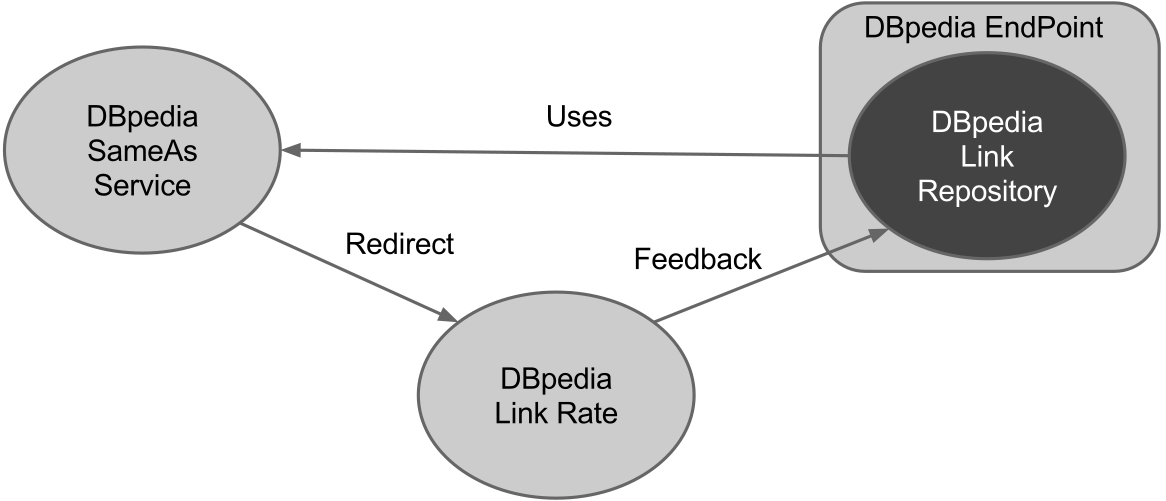
\includegraphics[width=\columnwidth]{img/contribution.png}
  	\caption{Relation of the contributions.}
  	\label{fig:contrib}
\end{figure}

Where the DBpedia Link Repository uses the DBpediaSameAs service in order to tackle the heterogeneity and giving the appropriate DUI, that redirects the user to the DBpedia Link Rate interface, thus, providing a feedback to the DBpedia Link Repository, therefore, improving the quality of the DBpedia endpoint.

\subsection{Evaluation}\label{ev:dbpediasameas}

The aim of this qualitative evaluation was centered in verifying the behavior of the service DBpediaSameAs, the Graphical User Interface (GUI) that gives the possibility to verify and rate the links.

There are chosen 3 evaluation criteria:

(1) \textbf{Normalization on DBpedia URIs}: With this criteria was evaluated if the DBpediaSameAs can provide an normalization on DBpedia URIs.
(2) \textbf{Rate the Links}: Where was evaluated if the DBpediaSameAs can provide a way to rate the links.
(3) \textbf{DBpediaSameAs as service}: Was evaluated if DBpediaSameAs can provide a stand alone service on the web that brings the normalization on DBpedia URIs.

\subsection{Normalization on DBpedia URIs}
The criteria used in this evaluation are uniquely to tackle heterogeneity, that was observed during the search of co-references between different data sets with a problem about redundancies.

When was used a URI from freebase in order to obtain a DBpedia URI was observed that at least 3 URIs were returned, that drives to the same final address.

As an example of a real case, executed in our public server, with a URI from Freebase:

\begin{lstlisting}
$ curl http://dbpsa.aksw.org/SameAsService/SameAsServlet?uris=http%3A%2F%2Frdf.freebase.com%2Fns%2Fm.015fr

returns: http://dbpedia.org/resource/Brazil
\end{lstlisting}

% \url{http://dbpsa.aksw.org/SameAsService/SameAsServlet?uris=http://rdf.freebase.com/ns/m.015fr}
% returns: \url{http://dbpedia.org/resource/Brazil}

Where, in this case, instead of 17 URIs from DBpedia, that goes to the same final address, our approach drives the user directly to the final address.

As can be observed on the figure~\ref{fig:transient} that approach the transitive and redirect URIs, where show that with this approach instead of have several URIs the user can have only one from the DBpediaSameAs. Thus, in this way, providing a normalization on DBpedia URIs.

\subsection{Rate the links}

In order to have a link rating, were implemented a GUI that allows the users to give some feedback, suggestions, in this way, improving the quality of the links.
The rate is a quite simple process, the GUI just ask the user to rate the link with +1 if the link attends your expectations or -1 if the link is wrong or some type of spam.
The GUI was developed using concepts from prefix.cc \footnote{Link to the official web site: \url{http://prefix.cc}} and work from Zaveri\cite{anra2013} such our system of rate (+1 and -1) and the standard of the web documents. Some improvements and personalization, also was provided, such as the suggestions and the possibility to check the link. The figure~\ref{fig:rate} shows the moment when the user clicked on the -1 and  indicated that the user didn't like the link and was asked to make a suggestion of a new URI.

\begin{figure}[hbt] 
  	\centering
	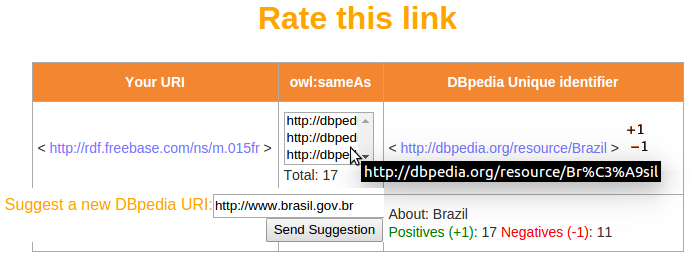
\includegraphics[width=\columnwidth]{img/rate2.png}
  	\caption{Rate a link.}
  	\label{fig:rate}
\end{figure}

The field about a suggestion for a new link will only appear when the user are not satisfied with the current link, then, when clicking on the -1, then the system will ask for an optional suggestion.

\subsection{Results}
The results of this work could also be expressed in numbers that was obtained during importing triples to the relational database and with some results from the sameAs.org web site.
A total of 62,531,487 triples imported into our database, the time was 2,220 seconds for the whole operation, thus, was noticed that 28,167 triples were imported per second.
The source code used to obtain the results is available in our github repository\footnote{Link to the source code: \url{https://github.com/firmao/dbpedia-links/blob/master/CreateDB.sh}}.

\subsubsection{Transitive and Redirect Links}
Transitive and Redirect Links are redundancies at DBpedia that supposed has a link to the same place, in other words, they use \qname{owl:sameAs} property, this links will redirect another links, will provide a transition between the links, that's why the name transitive.
In this case, instead of using this transitive links that points to the same final destination URI, this final destination URI will be used directly. The figure~\ref{fig:transient} try to make more clear this explanation.

\begin{figure}[hbt] 
  	\centering
	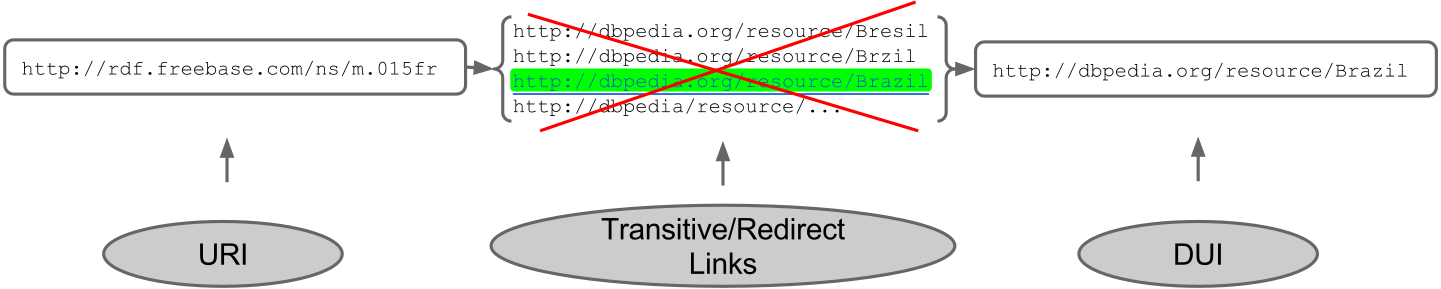
\includegraphics[width=\textwidth]{img/transient.png}
  	\caption{Transitive / Redirect links in DBpedia.}
  	\label{fig:transient}
\end{figure}

Was discovered and treated 6,473,988 triples with transitive and redirect links from 62,531,487 imported links among 142 domains inside DBpedia. Then, 10.35\% of the links can be avoided in some cases. 

\subsection{Discussion}
The DBpediaSameAs was evaluated with its normalization of URIs, link rate, and DBpediaSameAs as a stand alone service on the web.
As results of the normalization a DUI was obtained in order to tackle the heterogeneity. In other words, instead of several URIs  e.g. from sameAs.org one DUI was obtained.
The link rate functionality further allows to improve the quality of the dataset.

Despite, the GUI of DBpediaSameAs, also a stand alone service on the web was developed that brings the functionality to get a DUI without a GUI for agents or people which don't need to use the DBpediaSameAs in a Graphical mode, allowing use as an off-the-shelf component.

